\documentclass[12pt,brazil]{book}
\usepackage{babel}
\usepackage[utf8x]{inputenc}
\usepackage[top=2.5cm,left=2.5cm,bottom=2.5cm,right=2.5cm]{geometry}
\usepackage{url}
\usepackage{graphicx}
\usepackage{html}

\newcommand{\sep}{$\rightarrow$}

\title{Genoslab Handbook}
\author{Pedro Kröger}

\begin{document}
\graphicspath{{figs/}}

\maketitle

\begin{htmlonly}
  Baixe a versão em pdf \htmladdnormallink{aqui}
  {http://genos.mus.br/handbook/genoslab-handbook.pdf}.
\end{htmlonly}

\tableofcontents

\part{Introdução}
\label{part:introducao}

% TODO
% \chapter{Como contribuir para esse documento}
% \label{sec:como-contribuir-para}

\part{Ferramentas}
\label{part:ferramentas}

\chapter{Repositórios debian}
\label{cha:repositorios-debian}

Para instalar o csound5 você deve usar o pacote debian do Genos. Para
isso coloque a seguinte linha no seu \texttt{/etc/apt/sources.list}
(como root):

\begin{verbatim}
deb http://genos.mus.br/ debian/
\end{verbatim}

Em seguida rode o comando

\begin{verbatim}
aptitude update
\end{verbatim}

Agora você pode instalar os programas disponíveis no genos digitando
algo como o comando abaixo como root.

\begin{verbatim}
aptitude install <nome do programa>
\end{verbatim}

\chapter{Git}
\label{cha:git}

\section{Introdução}
\label{sec:introducao}

O Git (o ``g'' é pronunciado como na palavra gato e não como ``jit'')
é um programa para controle de versão distribuído desenvolvido por
Linus Torvalds (o criador do Linux) e mantido por Junio C Hamano. A
página do git em \url{http://git.or.cz/} tem vários tutoriais e
manuais.

\section{Instalação}
\label{sec:instalacao-3}

Para instalar o git no debian execute o seguinte comando.

\begin{verbatim}
aptitude install git-core git-completion git-doc git-gui gitk ssh
\end{verbatim}

É uma boa idéia configurar o git para usar o seu nome e email:

\begin{verbatim}
git config --global user.name "Seu Nome"
git config --global user.email "seu@email.com.br"
\end{verbatim}

\section{Repositórios do genos}
\label{sec:acesso-de-escrita}

O genos mantém diversos repositórios listados em
\url{git.genos.mus.br}. Para ter acesso de escrita você precisa criar
uma chave pública de criptografia. Para isso rode o comando:

\begin{verbatim}
ssh-keygen -t rsa
\end{verbatim}

Esse comando vai fazer uma série de perguntas como o tamanho da chave,
seu nome e email, etc. Se você não souber a resposta para alguma
pergunta não precisa se preocupar, o valor padrão deve ser o
suficiente. Quando ele pedir uma passphrase, certifique-se que você
não vai esquecê-la! A chave pública vai ser geradad no arquivo
\texttt{~/.ssh/id\_rsa.pub}. Para ter acesso de escrita nos
repositórios do genos envie o arquivo para Pedro Kroger.

Se você enviou a chave pública e seu acesso foi liberado, você pode
baixar um projeto no repositório do genos com o comando abaixo:

\begin{verbatim}
git clone ssh://cons@genos.mus.br/repos/<nome do projeto>
\end{verbatim}

Por exemplo, para baixar o projeto analise-harmonica você deve
digitar:

\begin{verbatim}
git clone ssh://cons@genos.mus.br/repos/analise-harmonica.git
\end{verbatim}

Contudo, se você não tem acesso de escrita ao repositório, ou seja,
não tem permissão para modificar o repositório diretamente, você ainda
pode baixar um projeto e contribuir mudanças (veja a seção
\ref{sec:enviando-patches}). Para isso baixe o repositório com o
comando abaixo:

\begin{verbatim}
git clone http://genos.mus.br/repos/<nome de repositório>
\end{verbatim}

\section{Comandos básicos}
\label{sec:comandos-basicos}

Você deve gravar suas mudanças com

\begin{verbatim}
git commit
\end{verbatim}

E enviar suas mudanças para o repositório central com o comando:

\begin{verbatim}
git push
\end{verbatim}

Para atualizar sua cópia local, ou seja, para baixar as mudanças que
outros tenham feito no repositório, use o comando:

\begin{verbatim}
git pull
\end{verbatim}

Revertendo mudanças que não foram enviadas.

\begin{verbatim}
git checkout -f
\end{verbatim}

\section{Usando diferentes ramos}
\label{sec:usando-o-git}

Para ver os ramos do repositório basta usar o comando

\begin{verbatim}
git branch
\end{verbatim}

Para mudar de ramo usa-se o comando

\begin{verbatim}
git checkout
\end{verbatim}

Mudando do ramo master para novo-ramo:

\begin{verbatim}
git checkout novo-ramo
\end{verbatim}

Conferindo o novo ramo:

\begin{verbatim}
git branch
  master
* novo-ramo
\end{verbatim}

Para criar um novo ramo e mudar para ele automaticamente usa-se

\begin{verbatim}
git checkout -b novo-ramo
\end{verbatim}

Para enviar um novo ramo para o repositório remoto:

\begin{verbatim}
git push origin ramo-local:ramo-remoto
\end{verbatim}

Para listar os ramos em um repositório remoto

\begin{verbatim}
git branch -r
\end{verbatim}

Para baixar um ramo no repositório remoto usa-se \texttt{git branch}
com a opção \texttt{--track}, indicando qual o nome do ramo local e o
nome do ramo remoto. É uma boa prática ter o mesmo nome para os ramos
local e remoto.

\begin{verbatim}
git branch --track novo-ramo origin/novo-ramo
\end{verbatim}

O nome \texttt{origin} nada mais é que um alias para a localização de
um repositório. Essa informação fica armazenada no arquivo
\texttt{.git/config} dentro do repositório. O trecho do
\texttt{.git/config} referente a configuração de \texttt{origin} pode
ser vista abaixo:

\begin{verbatim}
[remote "origin"]
        url = ssh://cons@genos.mus.br/repos/teste.git
        fetch = +refs/heads/*:refs/remotes/origin/*
\end{verbatim}

Veja na seção \ref{sec:o-arquivo-config} outras possibilidades de uso
para o arquivo \texttt{.git/config}.

Para manter os ramos atualizados, \texttt{git pull} e \texttt{git
  push} devem ser suficientes. O Git mantém cada ramo separado sem
interferir no outro. Contudo, mudanças sem commit vão aparecer em
todos os ramos.

Para mesclar as mudanças do branch \texttt{master} no seu ramo é só
fazer:

\begin{verbatim}
git pull .
\end{verbatim}

\section{Configuração}
\label{sec:configuracao}

\subsection{Usando abreviações}
\label{sec:usando-abreviacoes}

Eu sugiro que você coloque algo como a linha abaixo no seu
\texttt{~/.bashrc}.

\begin{verbatim}
export repos=ssh://cons@genos.mus.br/repos
\end{verbatim}

Desse modo você poderá baixar um projeto de uma maneira mais fácil:

\begin{verbatim}
git clone $repos/analise-harmonica.git
\end{verbatim}

\subsection{O arquivo config}
\label{sec:o-arquivo-config}

Você pode configurar o arquivo \texttt{.git/config} de um repositório
local para usar nomes abreviados. Isso é particularmente útil se está
usando mais de um repositório ou ramos diferentes.

\begin{verbatim}
cat >>.git/config <<EOF
[remote "public-repo"]
        url = ssh://yourserver.com/~you/proj.git
EOF
\end{verbatim}

Você pode fazer a mesma coisa com \texttt{git remote}:

\begin{verbatim}
git remote add public-repo ssh://example.com/project.git
\end{verbatim}

\subsection{Saída colorida}
\label{sec:saida-colorida}

Se você é viciado em saída colorida vai querer executar os comandos abaixo:

\begin{verbatim}
git config --global color.diff auto
git config --global color.status auto
git config --global color.branch auto
\end{verbatim}

\section{Enviando patches}
\label{sec:enviando-patches}

\part{Programas de áudio}
\label{part:programas-de-audio}

\chapter{CLM---Common Lisp Music}
\label{cha:clm-common-lisp}

\section{Pré-requisitos}
\label{sec:pre-requisitos}

Para compilar o CLM você precisará do gcc (o compilador C do projeto
GNU) e outras ferramentas instaladas. Além disso, o CLM não é um
programa auto-contido como o Csound. Ele é na verdade uma biblioteca
de funções Lisp. Para utiliza-lo você precisará de um compilador Lisp.
Eu recomendo o SBCL. Finalmente, você precisará de um bom editor. Eu
recomendo o Emacs com o Slime. O comando abaixo deve instalar tudo que
você precisa para começar:

\begin{verbatim}
aptitude install gcc emacs22 slime sbcl csh
\end{verbatim}

\section{Instalação}
\label{sec:instalacao}

Infelizmente não existe um pacote do CLM para o debian, então teremos
que instala-lo manualmente. Além disso, vamos instalar de uma maneira
que é mais fácil mas não é necessariamente robusta. Contudo essa
maneira é suficiente para você iniciar no programa. No futuro veremos
maneiras mais robustas de instalar o CLM.

Baixe a última versão do CLM no site do projeto em
\url{http://ccrma.stanford.edu/software/clm/} e descompacte o tar.gz
em um diretório. O diretório clm-3 será criado quando o arquivo for
descompactado. Os comandos abaixo efetuam essas operações:

\begin{verbatim}
wget ftp://ccrma-ftp.stanford.edu/pub/Lisp/clm-3.tar.gz
tar -xzf clm-3.tar.gz
\end{verbatim}

Em seguida coloque o seguinte código no final do arquivo
\verb|~/.swank.lisp|:

\begin{verbatim}
(defun clm ()
  (require :asdf)
  (setf *clm-dir* #p"/home/kroger/clm-3/")
  (push *clm-dir* asdf:*central-registry*)
  (asdf:operate 'asdf:load-source-op :clm)
  (setf *default-pathname-defaults* *clm-dir*))
\end{verbatim}

Observe que dentro do diretório clm-3 existem diversos arquivos. Os
arquivos com a extensão *.ins definem instrumentos do CLM e são os que
nos interessam. 

Para iniciar o CLM abra o emacs e slime com \texttt{M-x slime}. O REPL
(\textit{Read Eval Print Loop}) é o modo interativo de Lisp. Nele você
pode digitar expressões e obter resultados. Para programas maiores é
desconfortável entrar expressões no REPL, mas para testar coisas ele é
bastante útil. No REPL digite o comando abaixo para iniciar o CLM:

\begin{verbatim}
(clm)
\end{verbatim}

Sempre que você quiser usar o CLM basta iniciar o emacs, carregar o
slime e digitar ``(clm)'' no REPL.

Se você quiser iniciar o slime com uma tecla de atalho, coloque a
linha abaixo no seu \texttt{.emacs}:

\begin{verbatim}
(global-set-key [f9] 'slime)
\end{verbatim}

\section{Uso básico}
\label{sec:uso-basico}

Tendo compilado o CLM você pode carregar e usar instrumentos definidos
nos arquivos *.ins. Por exemplo, o arquivo v.ins define um instrumento
de nome ``fm-violin'' que sintetiza um violino usando FM. Você pode
carregar um instrumento com o comando abaixo:

\begin{verbatim}
(load "v")
\end{verbatim}

Finalmente, você pode usar o instrumento com o comando abaixo:

\begin{verbatim}
(with-sound () (fm-violin 0 1 440 .1)) 
\end{verbatim}

\section{Para saber mais}
\label{sec:para-saber-mais}

Para saber mais sobre a instalação do CLM veja o arquivo README.clm.
O manual está no arquivo clm.html. Ambos estão no diretório do CLM.

\chapter{Nyquist}
\label{cha:nyquist}

\section{Instalação}
\label{sec:instalacao-1}

Para instalar o nyquist é só usar o aptitude:

\begin{verbatim}
aptitude install nyquist
\end{verbatim}

O binário do nyquist se chama \texttt{ny}. Se você digitar \texttt{ny}
no terminal um prompt interativo vai abrir e esperar por comandos.
Você pode digitar algo simples para testar se o programa está
funcionando. O comando abaixo vai tocar um dó central:

\begin{verbatim}
(play (osc 60))
\end{verbatim}

\begin{htmlonly}
  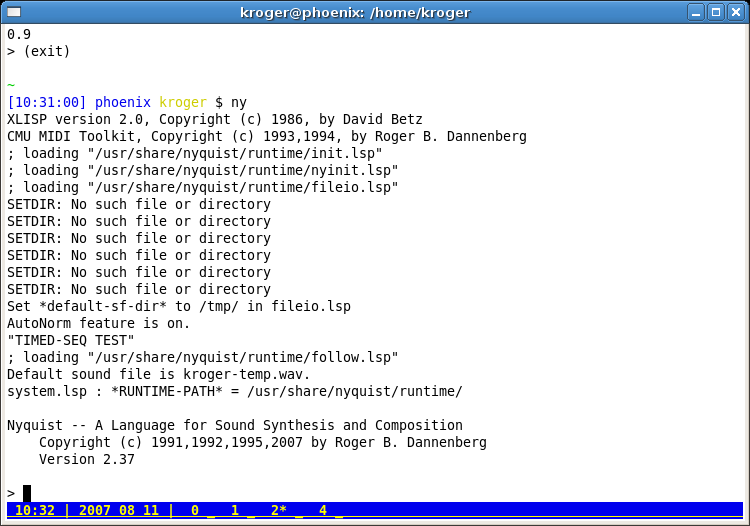
\includegraphics{ny1}
\end{htmlonly}

\begin{latexonly}
  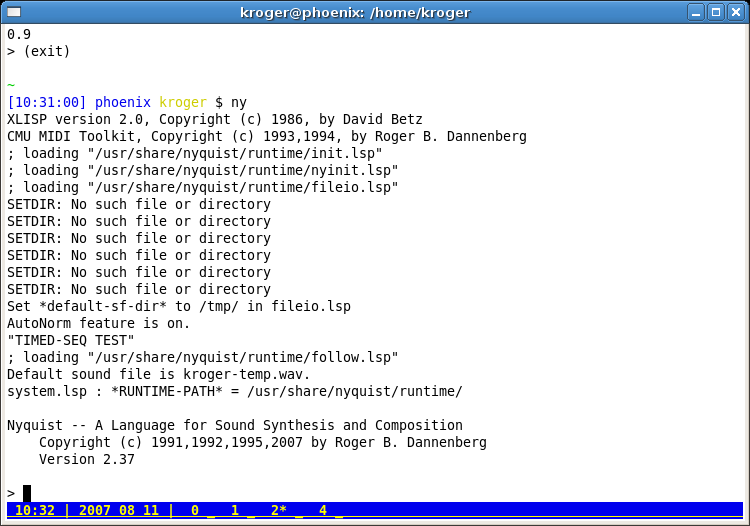
\includegraphics[scale=.5]{ny1}
\end{latexonly}

O manual do nyquist está disponível em
\url{http://www.cs.cmu.edu/~rbd/doc/nyquist/root.html} e em
\url{/usr/share/doc/nyquist/doc/home.html} se você instalou o pacote
debian.

\section{O modo para emacs}
\label{sec:o-modo-para-2}

Um modo preliminar do emacs para o nyquist pode ser encontrado em
\url{www.genos.mus.br/handbook/src/inf-nyquist.el}. Baixe o arquivo em
algum lugar no seu computador (eu sugiro \verb|~/lib/emacs/|) e
coloque as seguintes linhas no seu \texttt{.emacs}:

\begin{verbatim}
(autoload 'run-nyquist-lisp   "inf-snd" "Start inferior Snd-Lisp process" t)
(autoload 'nyquist-lisp-mode  "inf-nyquist" "Load nyquist-lisp-mode." t)
(setq inf-nyquist-lisp-program-name "ny")

(add-to-list 'auto-mode-alist '("\\.ny$" . nyquist-lisp-mode))

(add-hook 'nyquist-lisp-mode-hook
          (lambda ()
            (slime-mode nil)
            (local-set-key "\r" 'newline-and-indent)
            (setq lisp-indent-function 'common-lisp-indent-function)
            (setq indent-tabs-mode nil)))
\end{verbatim}

Todos os arquivos com a extensão \texttt{.ny} estarão associados ao
nyquist.

\section{Usando o nyquist com o emacs}
\label{sec:usando-o-nyquist}

Inicie o emacs e abra um arquivo com a extensão \texttt{.ny}, por
exemplo, \texttt{foo.ny}. Observe que o item ``Nyquist'' vai aparecer
no menu. Para iniciar o nyquist escolha no menu Nyquist\sep Start
Nyquist-lisp process ou \texttt{C-c C-s} no teclado. Um buffer chamado
\texttt{*Nyquist-lisp*} será aberto. Esse buffer é o modo interativo
do nyquist.

Você pode digitar comandos do nyquist no arquivo aberto (no nosso caso
\texttt{foo.ny}) e enviá-los para o nyquist com \texttt{C-x C-e} ou
através do menu em Nyquist\sep Send last Sexp.

\begin{htmlonly}
  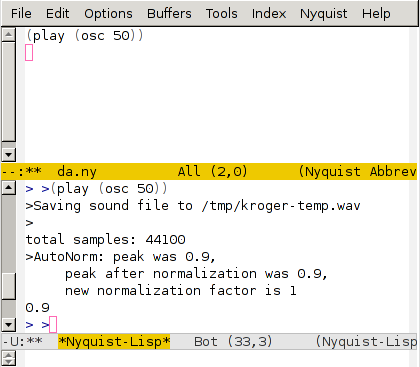
\includegraphics{ny2}
\end{htmlonly}

\begin{latexonly}
  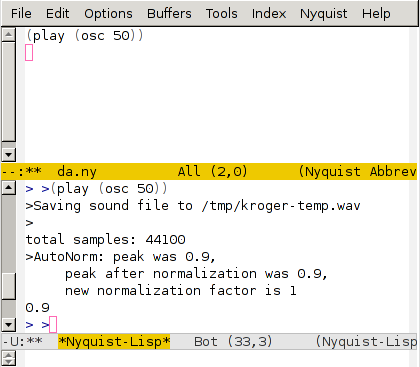
\includegraphics[scale=.5]{ny2}
\end{latexonly}

\section{Desenvolvendo plugins do audacity com o nyquist}
\label{sec:desenv-plug-do}

O audacity tem uma versão do nyquist embutida, de modo que plugins
podem ser desenvolvidos com ele. Os arquivos de plugins devem ser
colocados em \texttt{~/.audacity-files/plug-ins} e o audacity deve ser
reiniciado toda vez que um novo plugin for criado. 

Crie um arquivo \texttt{teste.ny} com o seguinte conteúdo:

\begin{verbatim}
;nyquist plug-in
;version 1
;type process
;name "Teste de fade in"
;action "Fading In..."
(mult (ramp) s)
\end{verbatim}

Observe que o efeito ``Teste de fade in'' vai aparecer no menu de
efeitos do audacity.

Um breve tutorial de como criar plugins do audacity com o nyquist pode
ser visto em \url{http://audacity.sourceforge.net/help/nyquist3}.

\chapter{SuperCollider}
\label{cha:supercollider}

O SuperCollider é uma linguagem de programação para síntese de áudio
em tempo real e composição algorítmica. A página do programa fica em
\url{http://supercollider.sourceforge.net}.

\section{Instalação}
\label{sec:instalacao-2}

Para instalar o supercollider no debian é só executar o comando
abaixo:

\begin{verbatim}
aptitude install supercollider supercollider-doc supercollider-server
\end{verbatim}

\section{Uso básico}
\label{sec:uso-basico-1}

Nós vamos usar o SuperCollider dentro do Emacs. Para ativar o modo
sclang que permite interagir com o SC coloque a seguinte linha no seu
\texttt{~/.emacs}:

\begin{verbatim}
(require 'sclang)
\end{verbatim}

O SuperCollider usar o jack para entrada e saida, então tenha certeza
de te-lo rodando antes de carregar o SC. Inicie o emacs e carregue o
modo sclang:

\begin{verbatim}
M-x sclang-start
\end{verbatim}

O emacs vai abrir dois \textit{buffers}, um chamado *SCLang:Workspace*
e outro *SCLang:PostBuffer*. No Workspace você pode digitar comandos
do SC. Os resultados dos comandos vão aparecer no PostBuffer.

O menu SCLang no emacs tem diversos comandos para lidar com o SC. O
mais importante é como parar um som que esteja tocando. Você pode
acessá-lo em SCLang$\leftarrow$Stop Main no menu, ou pelo teclado com
\texttt{C-c C-s}. Para computar uma linha de código use \texttt{C-c
  C-c } (ou \textit{Evaluate Line} no menu).

Para iniciar o servidor, digite a linha abaixo e, com o cursor em
qualquer lugar da linha, digite \texttt{C-c C-c}:

\begin{verbatim}
s = Server.local.boot;
\end{verbatim}

Agora compute a linha abaixo para tocar um lá continuamente (lembre de
usar o \texttt{C-c C-s} para parar o som).

\begin{verbatim}
{SinOsc.ar(442, 0, 0.2) }.play;
\end{verbatim}

Finalmente, para demonstrar o poder expressivo do SuperCollider, veja
o que é possível de fazer com uma única linha de código:

\begin{verbatim}
play{SinOsc.ar(OnePole.ar(Mix(LFSaw.ar([1,0.99],[0,0.6],2000,2000).trunc([400,600])*[1,-1]),0.98)).dup*0.1};
\end{verbatim}

\section{Para saber mais}
\label{sec:para-saber-mais-1}

O site do SuperCollider tem vários tutoriais na página
\url{http://supercollider.sourceforge.net/learning}.

\chapter{Csound}
\label{cha:csound}

\section{Instalação}
\label{sec:instalacao-4}

Para instalar o csound5 você deve usar o pacote debian do Genos. Veja
a seção \ref{cha:repositorios-debian} para ver como configurar seu
computador para usar o repositório de pacotes do Genos.

Tendo configurado o repositório do genos é só dar o comando abaixo
para instalar o csound.

\begin{verbatim}
aptitude install csound5
\end{verbatim}

Finalmente coloque a linha abaixo no seu \texttt{.bashrc}:

\begin{verbatim}
export OPCODEDIR=/usr/lib/csound/plugins
\end{verbatim}

\section{Uso básico}
\label{sec:uso-basico-2}

Para testar a instalação, crie um arquivo \texttt{teste.orc} com o seguinte
conteúdo:

\begin{verbatim}
instr 1
  a1        oscil     1000,440,1
            out       a1       
endin
\end{verbatim}

Crie também um arquivo \texttt{teste.sco} com o conteúdo abaixo:

\begin{verbatim}
f1  0 1024  10    1

i1 0 3
\end{verbatim}

Para usar o csound no terminal basta digitar \texttt{csound
  <orquestra> <partitura>}, por exemplo:

\begin{verbatim}
csound teste.orc teste.sco
\end{verbatim}

O csound vai gerar um arquivo de áudio chamado \texttt{teste.wav}.
Para ouvir em tempo real use a opção \texttt{-o}:

\begin{verbatim}
csound -odac teste.orc teste.sco
\end{verbatim}

Essa opção também pode ser usada para determinar o nome do arquivo de
áudio da saída:

\begin{verbatim}
csound -o teste.wav teste.orc teste.sco
\end{verbatim}

\section{O modo para emacs}
\label{sec:o-modo-para}

Um modo avançado e completo do csound para emacs está disponível em
\url{www.zogotounga.net/comp/csoundx.html}. Execute o comando abaixo
para baixar e descompactar o arquivo:

\begin{verbatim}
http://www.zogotounga.net/comp/stef-elisp-2.09.zip
unzip stef-elisp-2.09.zip
\end{verbatim}

Em seguida coloque as seguintes linhas no seu \texttt{.emacs}. Não
esqueça de trocar o diretório do comando \texttt{add-to-list} para o
diretório onde você baixou o modo.

\begin{verbatim}
(add-to-list 'load-path "/home/kroger/lib/emacs/stef-elisp/")
(require 'stef-elisp)
\end{verbatim}

A medida que você for customizando seu emacs, pode querer colocar
todas as extensões em um diretório específico. Eu sugiro
\verb|~/lib/emacs|.

\chapter{Snd}
\label{cha:snd}

\section{Instalação}
\label{sec:instalacao-5}

Para instalar a versão mais nova do snd configure seu computador para
usar o repositório de pacotes debian do genos. Veja como fazer isso na
seção \ref{cha:repositorios-debian}. Para instalar o snd é só digitar
o comando abaixo (como root):

\begin{verbatim}
aptitude install snd
\end{verbatim}

\section{O modo para emacs}
\label{sec:o-modo-para-1}

O snd é um programa para edição de áudio super poderoso. Ele é
completamente customisável usando scheme, um dialeto de lisp. Ele pode
ser controlado a partir do emacs. Para isso, baixe o arquivo
\url{www.genos.mus.br/handbook/src/inf-snd.el} para algum lugar no seu
computador (eu sugiro \verb|~/lib/emacs/|) e coloque as seguintes
linhas no seu \texttt{.emacs}:

\begin{verbatim}
(autoload 'run-snd-scheme   "inf-snd" "Start inferior Snd-Scheme process" t)
(autoload 'snd-scheme-mode  "inf-snd" "Load snd-scheme-mode." t)
(setq inf-snd-scheme-program-name "snd")

(add-to-list 'auto-mode-alist '("\\.snd$" . snd-scheme-mode))

(add-hook 'snd-scheme-mode-hook
          (lambda ()
            (local-set-key "\r" 'newline-and-indent)
            (setq lisp-indent-function 'common-lisp-indent-function)
            (setq indent-tabs-mode nil)))
\end{verbatim}

\section{Uso básico com o emacs}
\label{sec:uso-basico-3}

Inicie o jack e o emacs. Depois que o emacs iniciar, execute o comando

\begin{verbatim}
A-x run-snd-scheme
\end{verbatim}

Esse comando vai abrir o scheme e um modo interativo dentro do emacs.
Dentro do emacs abra um arquivo novo com a extensão \texttt{.snd}, por
exemplo, \texttt{teste.snd}. Observe que vai aparecer o menu
\texttt{Snd/Scheme} no menu do emacs. Como o snd tem o CLM embutido,
você pode fazer coisas semelhantes à seção \ref{cha:clm-common-lisp}.
Mas tenha em mente que no CLM estamos usando Common Lisp enquanto no
Snd estamos usando Scheme. Os dois são parecidos (são dialetos de
lisp) mas nem tudo que funciona em um funciona no outro. No arquivo
\texttt{teste.snd} digite o código abaixo:

\begin{verbatim}
(load-from-path "v.scm")
(with-sound () (fm-violin 0 3 440 .1))
\end{verbatim}

Você pode computar cada expressão no menu em Snd/Scheme\sep Send last
Sexp, ou usar \texttt{C-x C-e}. Observe que quando você carregar o
arquivo \texttt{v.ins} ele vai aparecer automaticamente no snd. Você
pode tocar o arquivo com \texttt{C-c C-p} e parar de tocar com
\texttt{C-c C-t}.

Você pode usar a função \texttt{do} para tocar um arpejo:

\begin{verbatim}
(with-sound ()
  (do ((i 0 (1+ i)))
      ((= i 8))
    (fm-violin (* i .25) .5 (* 100 (1+ i)) .1)))
\end{verbatim}

Assim como o CLM, os instrumentos são definidos com
\texttt{definstrument}. O instrumento abaixo toca uma senóide simples:

\begin{verbatim}
(definstrument (simp beg dur freq amp)
  (let* ((os (make-oscil freq))
	 (start (seconds->samples beg))
	 (end (+ start (seconds->samples dur))))
    (run
      (lambda ()
        (do ((i start (1+ i))) 
            ((= i end))
          (outa i (* amp (oscil os)) *output*))))))
\end{verbatim}

Para tocar o instrumento é só chamar a função \texttt{simp}:

\begin{verbatim}
(with-sound () (simp 0 3 440 .1))
\end{verbatim}

\end{document}
